\documentclass{pasa}%

\usepackage{graphicx}


\title[The Core-Cusp Problem Revisited: ULDM vs. CDM]{The Core-Cusp Problem Revisited: ULDM vs. CDM}

%% Please note that the command \and is not supported in \author.
\author[Emily Kendall and Richard Easther]{Emily Kendall$^1$, Richard Easther$^1$, \affil{$^1$Department of Physics, University of Auckland, Private Bag 92019, Auckland, New Zealand}}%


\jid{PASA}
\doi{10.1017/pas.\the\year.xxx}
\jyear{\the\year}


\usepackage{aas_macros}
\usepackage{hyperref} 
\hypersetup{colorlinks,citecolor=blue,linkcolor=blue,urlcolor=blue}

%%%%%%% IMPORTANT: We disable hyperlinks by default with this line, to avoid the error "\pdfendlink ended up in different nesting level" while writing.
\hypersetup{draft}
%%%%%%% You may comment or delete the line above to make hyperlinks in your paper active. If you then encounter a strange "\pdfendlink ended up in different nesting level than \pdfstartlink", don't worry! Uncomment the line again, and see https://www.overleaf.com/help/246 for further information.
% \usepackage{natbib}
\bibliographystyle{abbrvnat}
\setcitestyle{numbers,open={[},close={]}}

\begin{document}

\begin{frontmatter}
\maketitle

\begin{abstract}
The core-cusp problem is often cited as a motivation for the exploration of dark matter models beyond standard CDM [cold dark matter]. One such alternative model is ULDM [ultra-light dark matter]; extremely light scalar particles exhibiting wavelike properties on kiloparsec scales. ULDM dynamics are governed by the Schr\"{o}dinger-Poisson equations, which have solitonic ground state solutions consisting of gravitationally-bound condensates. Astrophysically realistic ULDM halos are predicted to consist of larger NFW-like configurations with a possible solitonic core, whose mass would be constrained by a core-halo mass relation. It has therefore been proposed that UDLM may naturally resolve the core-cusp discrepancy without recourse to baryonic physics. We describe a parameterisation for the radial density profiles of ULDM halos that allows for environmental variability of the core-halo mass relation. We then compare the semi-analytic profiles of ULDM and CDM and conclude that for halos up to $10^{12} M_\odot$ there exist feasible ULDM profiles which provide a diminished halo density at astrophysically accessible inner radii, thus ameliorating the core-cusp problem in theory. However, we then compare the theoretical profiles to observational data from the SPARC database, and conclude that while free parameters can be adjusted to provide reasonable fits to various subsets of the data, more comprehensive observational and simulation data, as well as better theoretical modelling of baryonic feedback is necessary before any robust conclusions can be drawn as to the suitability of either model.  

\end{abstract}

\begin{keywords}
Cosmology -- Core-Cusp Problem 
\end{keywords}
\end{frontmatter}


\section{INTRODUCTION }
\label{sec:intro}

It is widely agreed that non-baryonic dark matter constitutes the majority of the mass of the observable universe, but its precise nature remains an open question. Many dark matter models have been proposed, with particle CDM [Cold Dark Matter]  being the most widely studied. This scenario successfully accounts for the large scale structure of the universe \cite{Springel:2005nw} and the spectrum of anisotropies in the microwave background \cite{deBernardis:2000sbo, Hanany:2000qf, Halverson:2001yy, Netterfield:2001yq, Lee:2001yp, Ade:2015xua,  Hu:2001bc}, but the so-called ``small-scale crisis''  remains a challenge \cite{Weinberg:2013aya}. A key issue is the apparent tension between the  central density profiles of dark matter halos in simulations containing only gravitationally interacting CDM, and those inferred from observational data. Simulations tend to produce `cuspy' central density profiles \cite{Navarro:1995iw}, which grow as $1/r$ at small radii, but observational data appears to favour flattened central cores \cite{Moore:1994yx}. This so-called core-cusp problem has been the focus of much recent attention \cite{Dutton:2018nop, Read:2018pft, Genina:2018}. 
 
The seriousness of the core-cusp problem is the subject of ongoing debate, and may be ameliorated by adding baryonic matter to CDM simulations \cite{Benitez-Llambay:2018}. Nevertheless, the wider category of  ``small-scale'' problems in standard CDM along with tighter constraints from direct-detection experiments \cite{Schumann:2019eaa} motivates the study of alternative dark matter models. One scenario which has gained substantial traction is ultra-light dark matter [ULDM], also known variously as scalar-field dark matter, $\Psi$ dark matter, BEC dark matter and fuzzy dark matter. The lack of consensus regarding nomenclature can cause confusion, but it is sufficient to understand that all of the above names refer to models in which an extremely light scalar field constitutes the principal component of dark matter. It is for this reason such models are often referred to as `axion-like', since the QCD axion is a light scalar field familiar to most physicists. We prefer to use the designation `ULDM' in this work, emphasising the `ultra-light' nature of the scalar particle, for it is precisely this quality which gives rise to many of the characteristic features of this model.
As reviewed by Hui {\em et al.\/} \cite{Hui:2016ltb}, the very small ULDM particle mass ($\mathcal{O}(\sim 10^{-22}eV)$) corresponds to a kiloparsec-scale de Broglie wavelength. ULDM thus exhibits novel wave-like behaviour on astrophysically interesting scales and in particular can form soliton-like gravitationally confined Bose-Einstein condensates at these scales. ULDM simulations suggest that realistic astrophysical halos have an inner core consisting of a kiloparsec scale Bose-Einstein condensate or soliton, while the outer halo is a virialised system of scalar particles matching expectations from standard CDM \cite{Schwabe:2016rze, Veltmaat:2018dfz}. 

As the centres of ULDM solitons are flat, it would seem that this model could resolve the core-cusp problem without the inclusion of baryonic astrophysics. However, recent comparisons of theoretical halo profiles for both ULDM and CDM has lead to the suggestion that in some mass regimes ULDM actually exacerbates the core-cusp problem relative to CDM. The theoretical CDM profile used in this analysis is the NFW [Navarro-Frenk-White] profile \cite{Navarro:1995iw} characteristic of collisionless CDM, and often associated with WIMP [Weakly Interacting Dark Matter] CDM \cite{Robles:2018fur}. The theoretical ULDM profile combines a solitonic inner core, surrounded by an NFW outer halo. Because solitonic density profiles obey an inverse mass-radius scaling law, for massive cores it is plausible that the density of the ULDM halo might exceed that of an analogous NFW halo within a finite window of small radii. Indeed, the authors of Ref~\cite{Robles:2018fur} concluded that NFW profiles can actually outperform ULDM profiles for large dwarf galaxies (halo masses $M_h \gtrsim 10^{11} M_{\odot}$).  


In this work we examine the effect of scatter in the core-halo mass scaling relation and its implications for discussions of the core-cusp discrepancy in ULDM. Starting from the semi-analytic density profile of Ref.~\cite{Robles:2018fur} we look at the scatter in the parameters implied by Ref.~\cite{Schive:2014hza}, showing that this can ease concerns that the core-cusp problem is  exacerbated for ULDM relative to CDM for large dwarf galaxies. 

We discuss also the fact that semi-analytic models of halo density profiles fail to accommodate the effects of incoherent outer regions of ULDM halos which exhibit strong fluctuations, both temporally and spatially, as demonstrated through numerical modelling using tools such as the {\sc PyUltraLight} code \cite{Edwards:2018ccc}). Such fluctuations provide further evidence for the presence of intrinsic scatter in halo parameters at fixed mass, though detailed statistics of this scatter is yet to be determined. A further failing of the semi-analytic UDLM and NFW profiles is that neither make allowances for baryonic feedback, which is known to be significant for dwarf galaxies \cite{2018MNRAS.473.5698D, Benitez-Llambay:2018}. 

With these limitations in mind, we caution against attempting to discriminate between the applicability of ULDM and CDM models based on DM-only simplified theoretical profiles. Indeed, we find that for DM-only models, neither ULDM halos (for ULDM particle mass $0.8-2.5\times 10^{-22} \operatorname{eV}$)
nor NFW halos provide an overwhelmingly convincing fit to rotation curves of large dwarf galaxies, suggesting significant contributions from baryonic physics would be necessary for either model to yield a good fit to data. Here we use the SPARC database \cite{Lelli:2016zqa} to obtain galactic rotation curves. The details of this database will be discussed in following sections, but the curves for some dwarf galaxies are limited to a few data points over small ranges of radial distances, and many profiles have significant uncertainties, further complicating attempts to draw robust conclusions from this approach. 

Through comparison with the SPARC database, we show that one can fairly easily tailor the parameters of the ULDM model to yield a reasonable fit to data from galaxies which exhibit a steep decrease in rotation velocity at small radii, finding that a ULDM particle mass of $10^{-23}\operatorname{eV}$ appears superficially to provide such a fit, seemingly ameliorating the core-cusp discrepancy in these cases. This small ULDM particle mass, however, is in tension with some recent ULDM constraints. Hence, further multifaceted investigation is needed to determine whether ULDM provides a suitable framework to describe galactic density profiles. We use this example of parameter-fitting to demonstrate that it is unlikely to be meaningful to draw conclusions about the efficacy of either ULDM or CDM models based only on simplified DM-only theoretical density distributions, especially when relevant observational data is limited and statistics from numerical simulations lacking. 

The structure of the paper is as follows. In Section \ref{sec:models}, we review the construction of semi-analytic density profiles for both the ULDM and CDM models. and briefly discuss aspects of realistic ULDM halos which are not captured by the semi-analytic model. In Section \ref{sec:velocity} we compare the semi-analytic density profiles for ULDM and CDM halos in the dwarf galaxy mass range $10^{11} - 10^{12}\operatorname{M}_{\odot}$, taking into account statistical variation in both the NFW concentration parameter and the ULDM core-halo mass relation. We then compare the radial velocity profiles inferred from these density profiles with astrophysical data from the SPARC database \cite{Lelli:2016zqa}. We conclude in Section \ref{sec:conclusion}.

 
\section{Semi-analytic models of dark matter halos}\label{sec:models}


\subsection{The NFW profile of CDM}\label{sec:NFW}

We begin by looking at the semi-analytic parametrisations of ULDM and CDM halo models. The  well known  NFW   profile of CDM \cite{Navarro:1995iw, Maccio:2008pcd}  is given by
%
\begin{equation}\label{eq:nfw}
    \rho_\mathrm{NFW}(r)=\frac{\rho_0}{\frac{r}{R_s}\left(1+\frac{r}{R_s}\right)^2} \, .
\end{equation}
%
The parameters $\rho_0$ and $R_s$ vary from halo to halo; $\rho_0$ can be interpreted as a characteristic density, while $R_s$ is the scale radius and determines the radius at which the transition between the `small $r$' and `large $r$' limits occurs. At small radii the profile is proportional to $1/r$, while at large radii it goes as $1/r^3$.

The NFW halo is assumed to be radially symmetric, and requires truncation at a finite radius in order to avoid the divergence in the mass integral as $r\rightarrow \infty$. This is typically set by the virial radius, which is approximately determined via the spherical top-hat collapse model \cite{White:2000jv, Suto:2015jdt, Herrera:2017epn} describing the evolution of a uniform spherical overdensity in a smooth expanding background. Gravitational collapse of the overdensity halts when virial equilibrium is reached. The corresponding virial radius is the radius at which the mean internal density is $\Delta_c \rho_\mathrm{crit}(t)$. Here $\rho_\mathrm{crit}(t)$ is the critical density of the universe at time $t$. The numerical factor $\Delta_c$ is of order $10^2$ and while different conventions exist, we will take the common value of $\Delta_c = 200$ \cite{Richings:2018} in what follows. 

Once the virial radius is specified as the outer limit of the halo, equation \ref{eq:nfw} completely specifies the density profile for given  $\rho_0$ and $R_s$. For any given virial mass, there is a range of corresponding NFW density profiles, with the distributions of $\rho_0$ and $R_s$ emerging from the mass-concentration-redshift relation seen in N-body simulations and observations \cite{Ludlow:2013vxa, Ragagnin:2018enf}. 

\subsection{The piecewise ULDM halo profile}

ULDM dynamics is governed by the Schr{\"o}dinger-Poisson system of coupled differential equations. In a static background, they take the dimensionless form  
%
\begin{align}
    &i\dot{\psi} = -\frac{1}{2}\nabla^2\psi+\Phi\psi \\
    &\nabla^2\Phi = 4\pi \vert \psi\vert^2
\end{align}
%
where $\psi$ is the ULDM wavefunction, $\Phi$ is the Newtonian potential, and the density $\rho \propto |\psi|^2$. The solitonic ground state profile cannot be written down analytically, but given a numerically computed spherically symmetric  profile $\psi$ with $\psi(0)=1$, the full family of solutions is
%
\begin{equation}
    \psi'(x) = \gamma\psi(\sqrt{\gamma}x),
\end{equation}
%
where $\gamma$ is a scaling parameter and the dimensionless mass of the soliton is proportional to $\sqrt{\gamma}$, while the dimensionless radius is proportional to $1/\sqrt{\gamma}$. The dimensionless density $\vert\psi\vert^2$ and dimensionless radius $x$ can be transformed into dimensionful quantities by
\begin{align}
    \rho &= \mathcal{M}\mathcal{L}^{-3}\vert\psi\vert^2, \label{eq:density_conv} \\
    r &= \mathcal{L}x, \label{eq:mass_conv}
\end{align}
where
\begin{equation}\label{eq:length}
    \mathcal{L}=\left(\frac{8\pi\hbar^2}{3 m^2H_0^2\Omega_{m_0}}\right)^{\frac{1}{4}}\approx121\left(\frac{10^{-23}\operatorname{eV}}{m}\right)^{\frac{1}{2}}\operatorname{kpc},
\end{equation}
%
and 
%
\begin{align}\label{eq:mass}
    \mathcal{M}&=\frac{1}{G}\left(\frac{8\pi}{3 H_0^2\Omega_{m_0}}\right)^{-\frac{1}{4}}\left(\frac{\hbar}{m}\right)^{\frac{3}{2}}\nonumber\\
    &\approx 7\times 10^7\left(\frac{10^{-23}\operatorname{eV}}{m}\right)^{\frac{3}{2}}\operatorname{M}_{\odot}.
\end{align}



 
Ref.~\cite{Robles:2018fur} gives a piecewise parameterization of the generic ULDM profile 
%
\begin{equation}\label{eq:piecewise}
     \rho(r)=
    \begin{cases}
      \rho_{sol}(r), & 0\leq r \leq r_{\alpha} \\
      \rho_\mathrm{NFW}(r), & r_{\alpha}\leq r \leq r_{\mathrm{vir}},
    \end{cases}
\end{equation}
%
where $\rho_{sol}(r)$ is the appropriately scaled density profile of the ground state soliton solution. The contribution from the solitionic core and the overall virial mass is predicted to obey a scaling relationship \cite{Schive:2014hza, Chavanis:2019faf}, which sets the central density, $\rho_c$, of a ULDM halo with virial mass, $M_{\mathrm{vir}}$. This yields an expression relating the core size to the velocity dispersion, and finally to the halo virial mass.%
\footnote{The authors of \cite{Schive:2014hza} suggest the following general expression:
\begin{equation}
    M_c = \alpha \left(\vert E\vert/M\right)^{1/2},
\end{equation}
where the core mass $M_c$ is determined by the total energy, $E$, and the total mass of the halo, $M$ where $\alpha$ is a constant of order unity. They then explain that the right hand side of the equation represents the halo velocity dispersion, while the left hand side  represents the inverse core size due to soliton scaling laws. By invoking the virial condition of the spherical collapse model, the authors then  construct the redshift dependent relationship between the solitonic core mass and the halo virial mass for a ULDM halo.}

\begin{figure}[t]
\centering
\includegraphics[scale = 0.6, trim={1cm 0cm 0cm 0.4cm}]{slice.eps}
\caption{Illustration of the scale of the fluctuations present in the incoherent outer halo for a merger of 8 randomly located solitons. The contour plot represents the ($\mathrm{log}_{10}$ scaled) local density across a slice through the centre of the final halo. In this plot, distance is not log-scaled, and we see that the spatial size of the fluctuations is of the same order of magnitude as the solitonic core itself.}\label{fig:contour}
\end{figure}
%
The core-halo mass relation can also be understood simply by matching the virial velocities of the core and the wider halo (see Appendix \ref{app:core-halo} for details). 
At $z=0$ the relationship is found to be \cite{Schive:2014hza} 
%
\begin{equation}\label{eq:central_dens}
    \rho_c = 2.94\times10^6 \operatorname{M}_{\odot}\operatorname{kpc}^{-3}\left(\frac{M_{\mathrm{vir}}}{10^9 M_{\odot}}\right)^{4/3}m_{22}^{2},
\end{equation}
and 
\begin{equation}
    r_c = 1.6 \operatorname{kpc}\left(\frac{M_{\mathrm{vir}}}{10^9 M_{\odot}}\right)^{-1/3}\frac{1}{m_{22}},
\end{equation}
%
where $r_c$ is the radius at which the density is half of the central value, and $m_{22}$ is given by $m_{22} \equiv m / 10^{-22} \operatorname{eV}$ where $m$ is the ULDM particle mass. 

While the piecewise semi-analytic ULDM profile is a useful tool, one should be mindful of its inherent limitations. For example, while a number of studies have attempted to establish the `universal' properties of ULDM halos, many of these studies generated ULDM halos through the merger of several smaller compact objects such as solitons \cite{Schwabe:2016rze, Mocz:2017wlg}. This method of assembling halos is not necessarily representative of a realistic structure formation process. However, these methods of simulating ULDM halos persist due to the computational difficulty of undertaking large-scale cosmological simulations. For this reason, there exists limited data from which to draw robust conclusions about the properties of ULDM halos originating due to gravitational collapse in the early universe. 
Indeed, there is much more to be investigated in this arena. In particular, more work needs to be done in order to understand the characteristic timescales associated with the formation of quantum pressure supported cores in different scenarios, including condensation from a fluctuating background, gravitational collapse in an expanding background, and mergers of objects with and without stable central cores. Until the dynamical timescales of core formation are fully understood for halos of a wide range of masses, we must be cautious when extrapolating the core-halo mass relation  assumed in this semi-analytic halo model to realistic halos in regions of parameter space which have yet to be explored numerically. It should also be acknowledged that it is difficult to accurately predict the effect that baryonic feedback will have on the formation of solitonic cores in halos of different masses, though one expects this effect to be significant at small radii, and therefore non-negligible in the present context.

One must also acknowledge that the semi-analytic model presented above does not take into account halo substructure. It is clear from simulations of soliton mergers that resulting halos exhibit turbulent outer regions, with fluctuations on scales comparable to the core size. This is illustrated in Figure \ref{fig:contour}. In addition to the fluctuations inherent in a large ULDM halo, we would also expect to see smaller halos orbiting larger halos at a variety of scales, as is also predicted in CDM models. Clearly this sort of substructure cannot be captured by the semi-analytic model described here, and therefore predictions for tracer velocity profiles cannot be expected to match accurately with realistic astrophysical objects, particularly when there are a small number of tracer objects from which to infer global properties. Furthermore, not only are spatial fluctuations not properly accounted for by the semi-analytic model, but temporal fluctuations in the core density are also not captured. Such fluctuations arise because halo cores are not exact soliton solutions of the Schr\"{o}dinger-Poisson equation, rather they interact non-trivially with the fluctuating NFW-like outer halo, and as such their central densities can vary with time by as much as a factor of two \cite{Veltmaat:2018dfz}.

These limitations discussed here therefore suggest that the core-halo mass relation of the semi-analytic model should not be interpreted as an inviolable rule, but rather a statement about the averaged characteristics of a statistical distribution. To account for this, for a given virial mass, we consider a range of possible central densities (one might consider this in some sense analogous to the scatter in NFW concentration parameters \cite{Maccio:2008pcd}). We base our choice of range on the results of \cite{Schive:2014hza}, which indicate a scatter of up to $\pm 50\%$ in the core mass $M_c$ for a given virial mass. We note, however, the small sample size and limited halo mass range ($ M_{\mathrm{vir}} \approx 10^8-10^{11} \operatorname{M}_{\odot}$) considered in ~\cite{Schive:2014hza}  mean that a detailed statistical distribution of the properties of realistic astrophysical halos cannot yet be determined. Hence, in the present analysis we will assume a scatter of $\pm 50\%$, but note that future simulations (especially those including baryonic feedback) will lead to improved predictions for this distribution. 

To further account for statistical variation in halo characteristics, we allow for variation in the radius at which the solitonic profile of the ULDM halo transitions into an NFW profile. This is acknowledged in \cite{Robles:2018fur}, and is captured by the parameter $\alpha$, such that the transition radius, $r_{\alpha}$, is given by $r_{\alpha} = \alpha r_c$, where $3 \leq \alpha \leq 4$. The chosen value of the radius of transition will of course affect the parameters of the theoretical outer NFW halo, in particular the scale radius, as the core-halo mass relation should be maintained as the transition radius is varied.

With the allowances for statistical variation in both the central soliton density and the transition radius taken into account, we can create a range of plausible ULDM halo profiles for a given halo virial mass. To do this, we use the virial mass to predict $\rho_c$, and then allow the range of densities within $\pm 50\% $ of this central value. Combining the central density with an assumption for $\alpha$, the solitonic piece of the ULDM profile is then completely specified, and its mass can be calculated. From here, we can calculate the remainder of the virial mass which must be accounted for by the NFW tail of the profile. Then, by matching the densities of the NFW tail and the inner soliton at the transition radius, the values of the $R_s$ and $\rho_0$ parameters of the ULDM profile NFW tail are fully constrained.  

In summary, we stress that while we have made attempts to account for statistical variation in halo parameters, one cannot expect this simplified semi-analytic model of ULDM halo structure to accurately represent real astrophysical objects, and we must therefore be careful when using such models to draw conclusions as to the relative performance of the ULDM model and the CDM model of dark matter. Likewise, it is known that the NFW profile does not accurately represent CDM models when baryonic feedback is included, and this further limits the utility of a direct comparison of our two semi-analytic profiles with observational data. 


\section{ULDM and CDM halos and astrophysical data}\label{sec:velocity}

\begin{figure*}[t]
\centering
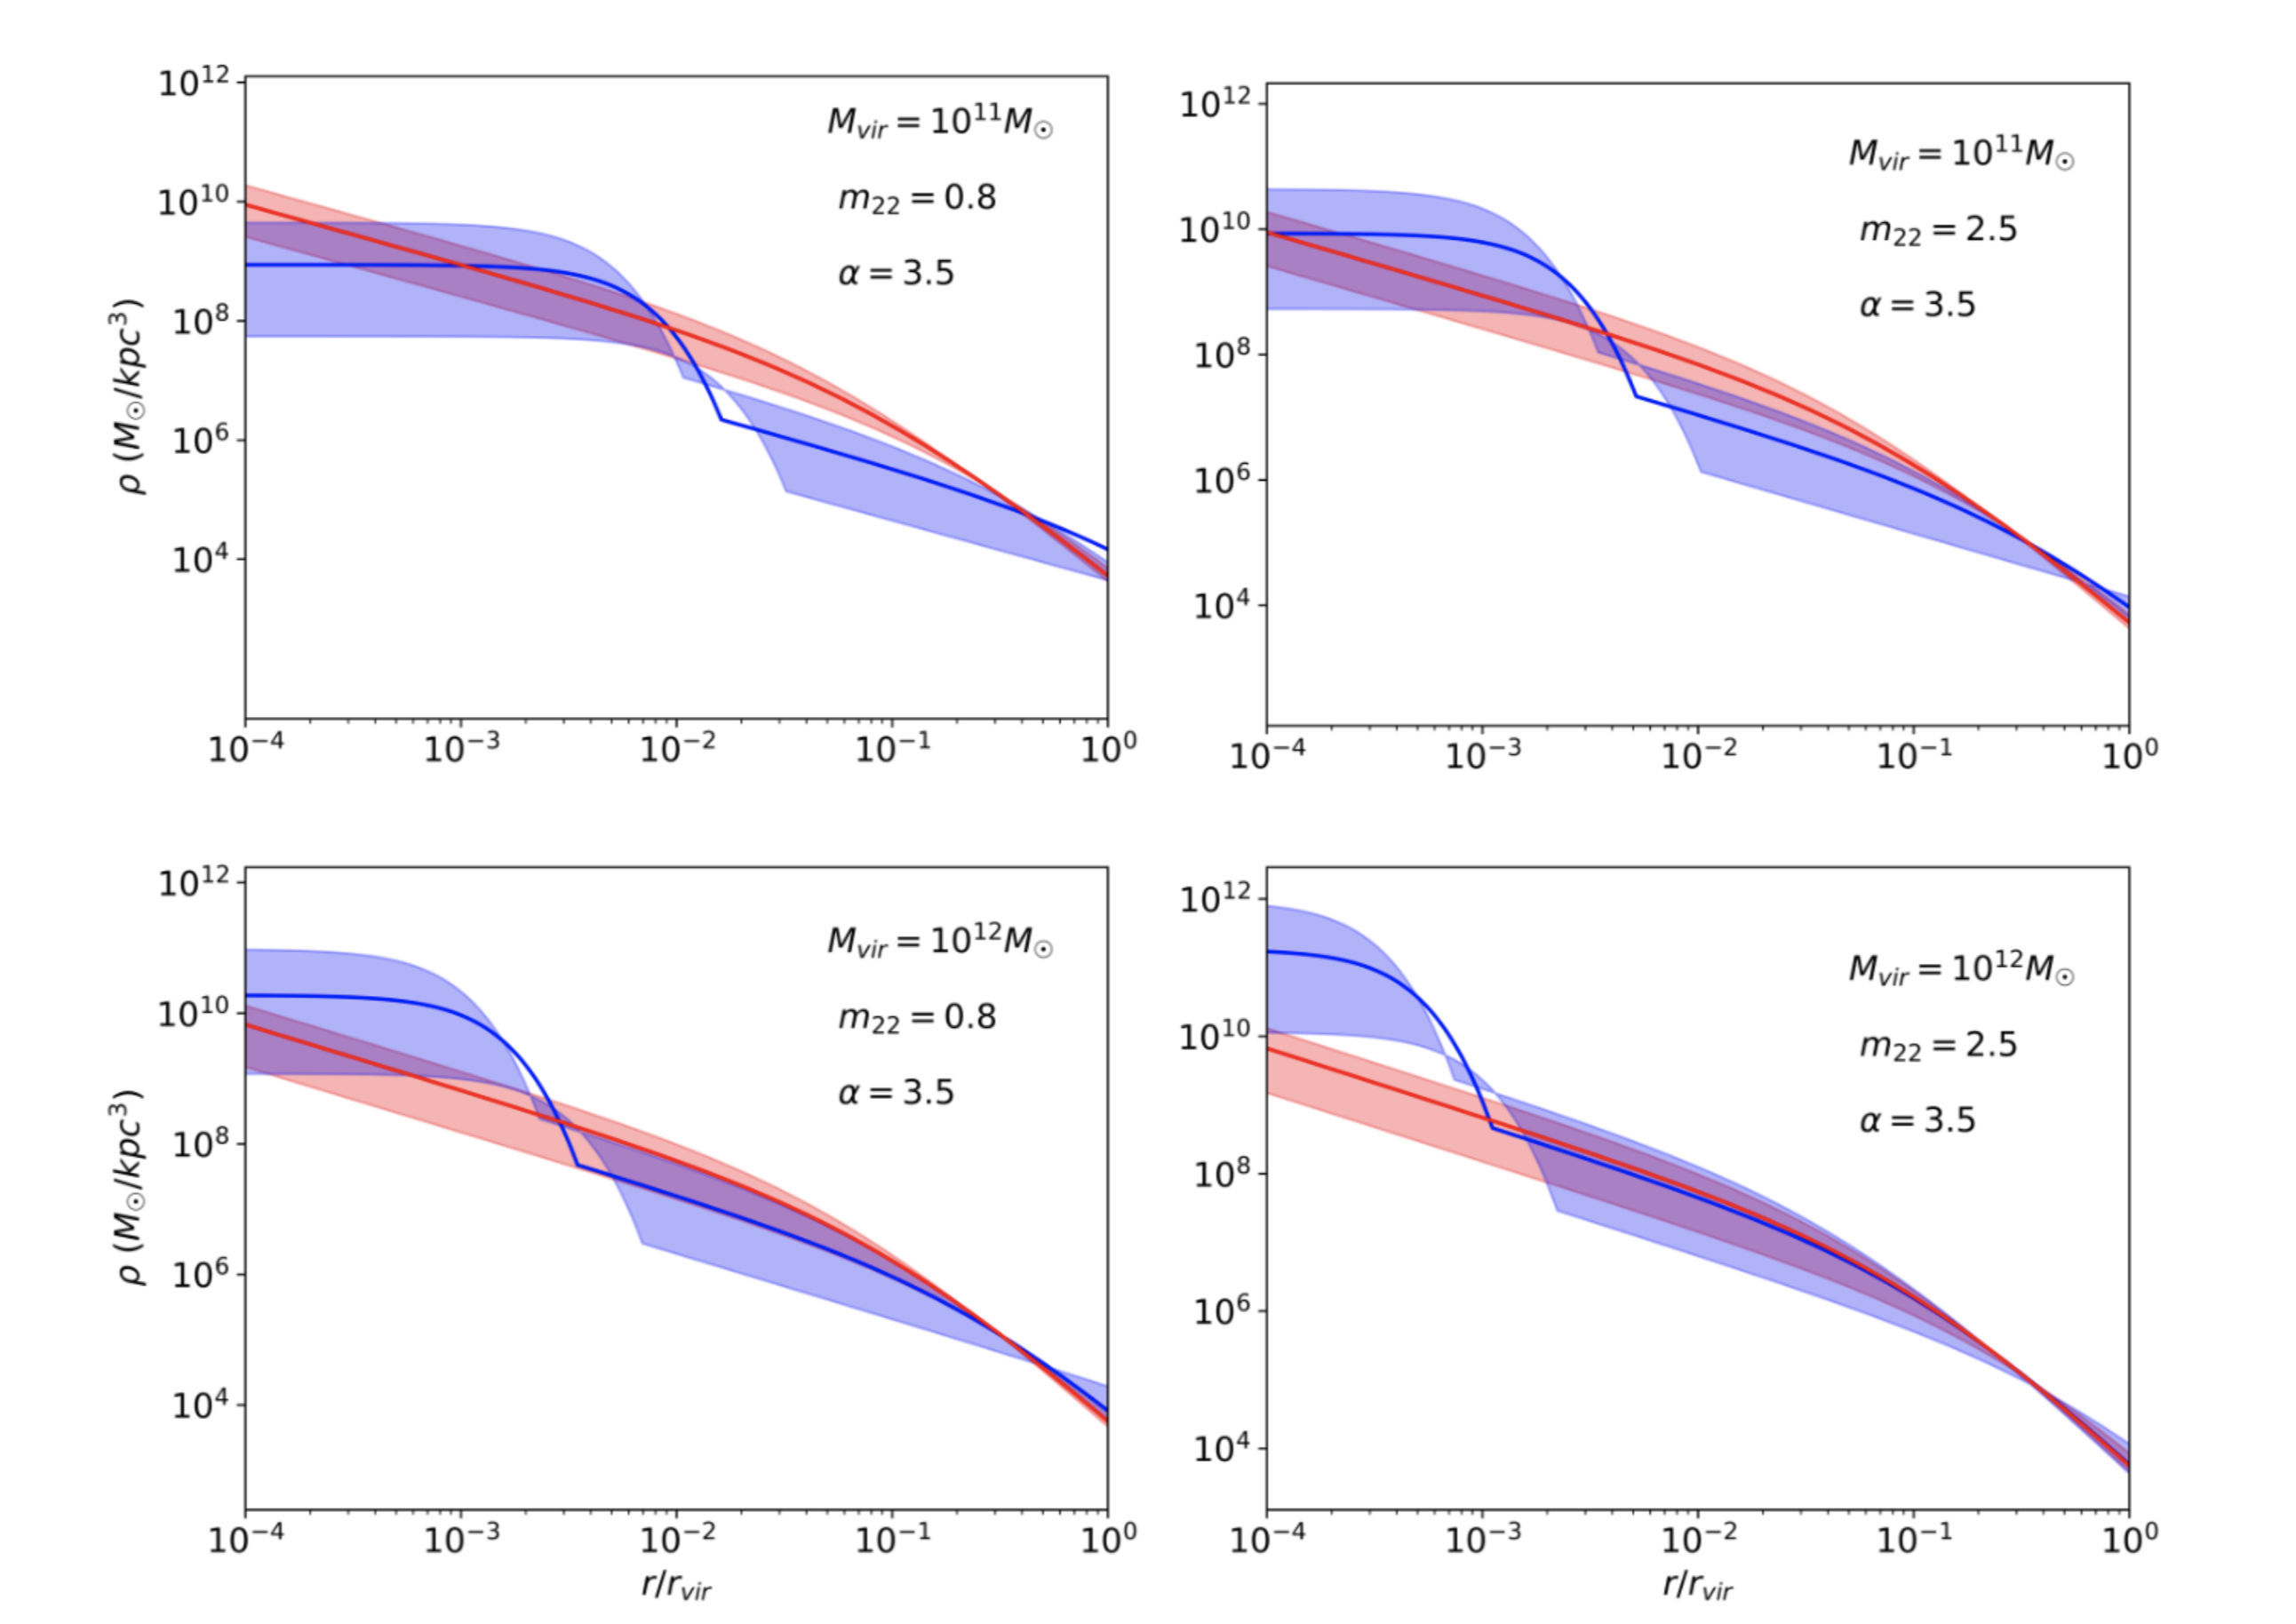
\includegraphics[scale=0.4, trim={2cm 0cm 0cm 1cm}]{new_combined_1.png}
\caption{Density profiles as a function of radius (normalised to the virial radius) for ULDM and NFW halos of masses $10^{11}\operatorname{M}_{\odot}$ (top) and $10^{12}\operatorname{M}_{\odot}$ (bottom). The left panel represents the results for $m_{22} = 0.8$, while the right panel corresponds to $m_{22}=2.5$. The transition radius is fixed at $r_{\alpha} = 3.5*r_c$ as this value lies in the middle of the expected theoretical range and its value does not affect the value of the ULDM central density. The blue shaded region represents the ULDM profile with $\operatorname{M}_c = \operatorname{M}_{\mathrm{cp}} \pm 50 \% \operatorname{M}_{\mathrm{cp}}$, while the solid blue line represents the ULDM profile when the theoretical core-halo mass relation is taken to be exact. The red shaded region represents the range of NFW profiles for a halo of the same virial mass with a 2$\sigma$ variation around the median (solid red line).}\label{fig:profiles}
\end{figure*}
 
Using the semi-analytic profiles described above, we now compare the radial profiles of ULDM halos to NFW halos. We focus on masses in the range $10^{11}$ and $10^{12} \operatorname{M}_{\odot}$ since these cases showed an apparent worsening of the core-cusp problem in Ref.~\cite{Robles:2018fur}. Figure \ref{fig:profiles} shows comparisons for representative masses; the shaded blue region represents the ULDM halos whose scatter in the core-halo mass relation is given by $\operatorname{M}_c = \operatorname{M}_{\mathrm{cp}} \pm 50 \% $ range, where $\operatorname{M}_{\mathrm{cp}}$ is the theoretical predicition for the core mass. Due to the  Schr{\"o}dinger-Poisson soliton scaling relations, this mass range corresponds to a range of $ \gamma_p /4 \leq \gamma \leq 9\gamma_p/4$, where $\gamma_p$ is the theoretical prediction of the square root of the dimensionless central density, implying a large variation in the central density and widely varying predictions for the overall ULDM profiles. In each case we have chosen a transition between the solitonic to NFW region at $\alpha = 3.5$, as this value lies in the middle of the predicted range, and does not affect the central density (the core lies well within the solitonic region). Meanwhile, the red shaded regions of Figure \ref{fig:profiles} show the $2\sigma$ variation about the theoretical prediction for the concentration parameter of the corresponding NFW halo in each case \cite{Maccio:2008pcd}. 



Following Ref~\cite{Robles:2018fur}, we plot to a minimum radius of $r/r_{\mathrm{vir}} = 10^{-4}$ and for the same choices of $m_{22}$. We note in passing that for any $\operatorname{M}_{\mathrm{vir}}$, the NFW halo density at very small radii will inevitably exceed that of the ULDM halo, though the threshold for this transition may be arbitrarily small, and not observationally relevant. However, the apparent worsening of the core-cusp discrepancy does depend on the choice of inner radial cutoff.

From Figure \ref{fig:profiles} we see that for halo masses of $10^{11}\operatorname{M}_{\odot}$ there is a wide range of $M_c$ for which the ULDM profile is `less cuspy' than its NFW counterpart. For a halo mass of $10^{12}\operatorname{M}_{\odot}$ and a ULDM particle mass $m_{22}=0.8$ the range of plausible ULDM profiles likewise includes those which are `less cuspy' than the corresponding NFW profile. At higher particle mass ($m_{22}=2.5$) for $10^{12}\operatorname{M}_{\odot}$ halos, the NFW profiles tend to be less peaked than corresponding ULDM profiles at radial distances in  the range $10^{-4}\leq r/r_{\mathrm{vir}} \leq 1$. Whether or not the excess central density in this mass regime constitutes a problem depends upon a comparison with suitable observational data. 

In order to compare the theoretical profiles with data, we turn to the SPARC database. However, it is not the dark matter halo density profiles themselves that are extracted from astrophysical observations, rather it is the (line of sight) velocity distributions of tracer stars as a function of galactocentric radius. We must therefore transform our theoretical density profiles into velocity profiles to make the required comparisons. Of course, the effects of non-circular motion and kinematic irregularities constitute a non-trivial source of random error in observed velocities, which should be kept in mind especially when working with limited data sets. 

We convert our density profiles to velocity distributions \cite{Sofue:2008wt} via 
%
\begin{equation}
    V(r)^2 = \frac{4\pi G}{r}\int_0^r \rho(r')r'^2 dr',
\end{equation}
where 
\begin{equation}\label{eq:vel_decomp}
    V^2 = V_{\mathrm{disk}}^2 + V_{\mathrm{bulge}}^2 + V_{\mathrm{gas}}^2 + V_{\mathrm{halo}}^2.
\end{equation}
%

\begin{figure*}[t]
\centering
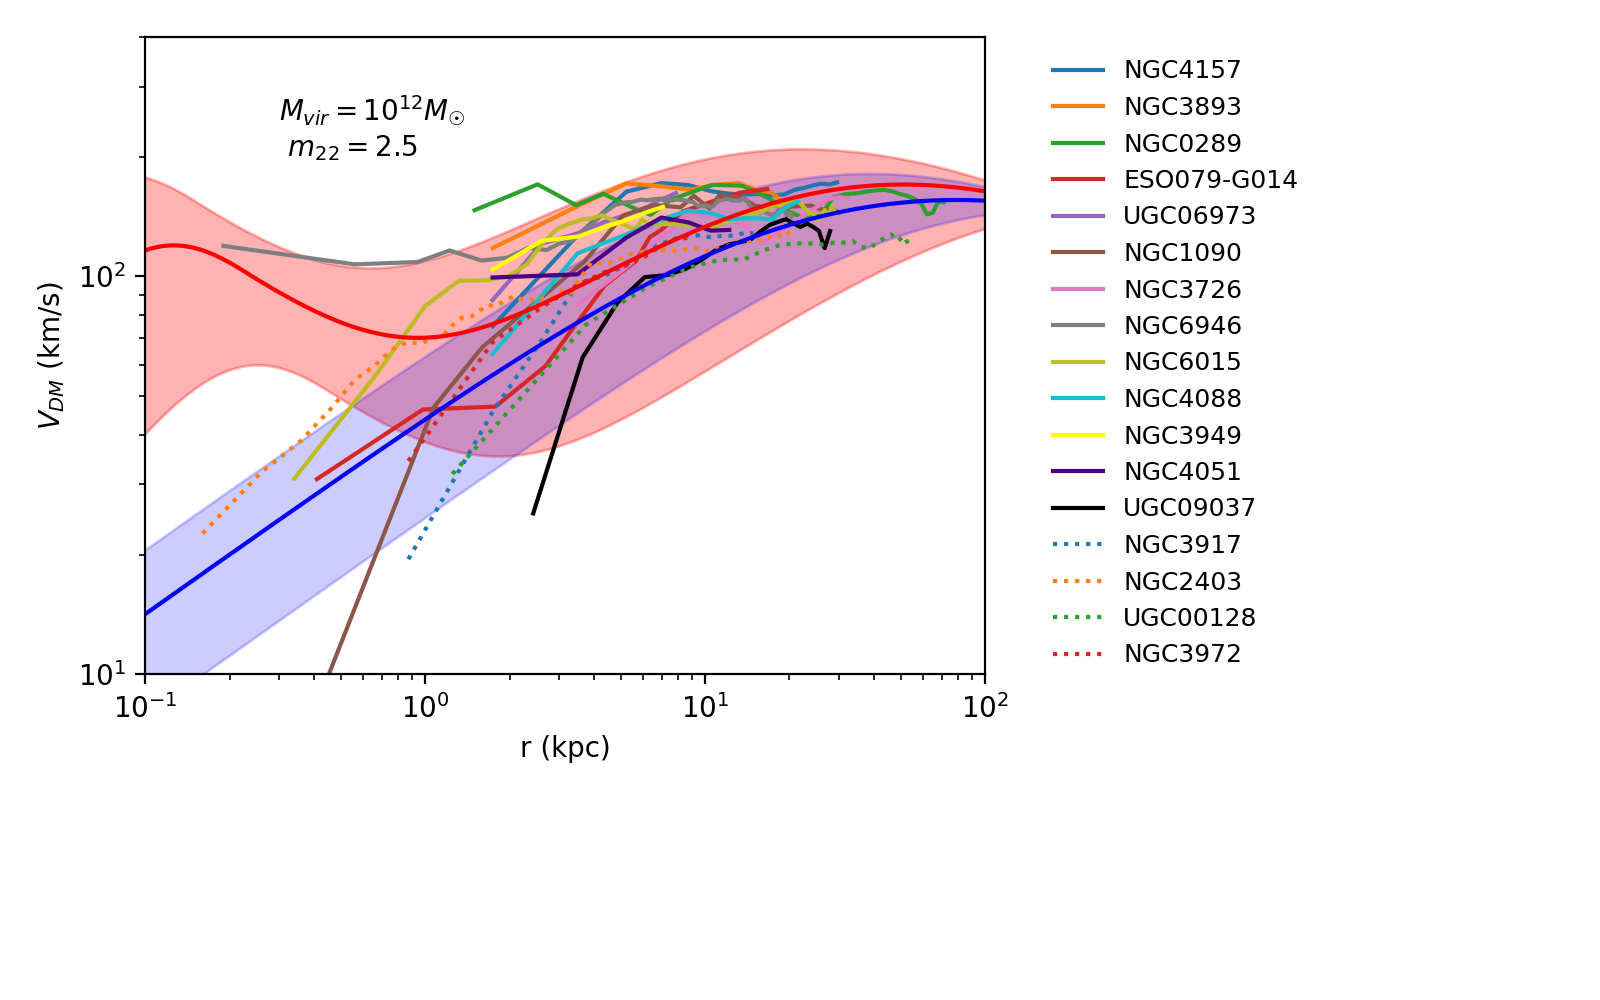
\includegraphics[scale=0.9, trim={0cm 2.5cm 3cm 0cm}]{000_vs_SPARC_10_12.png}
\caption{Velocity distributions for galaxies with maximum velocities in the range $125 \leq v < 175\operatorname{kms}^{-1}$ in the SPARC database. Data at innermost radii is limited for these galaxies, making it difficult to determine the overall characteristics of the profiles. The SPARC data is plotted along with theoretical NFW and ULDM profiles, assuming a virial mass of $10^{12} \mathrm{M}_{\odot}$, $m_{22} = 2.5$, and $\pm 50 \%$ scatter in the ULDM core-halo mass relation and $\pm2\sigma$ scatter in NFW concentration. Galaxies in the legend are ordered from highest maximum velocity (top) to lowest (bottom).}\label{fig:high_v}
\end{figure*}

We now compare this distribution to profiles in the SPARC database, which contains photometric data for 175 galaxies and rotation curves from $\mathrm{H}_{\mathrm{I}}$/$\mathrm{H}_{\alpha}$ studies. The disk and bulge velocities in the SPARC database are given for $\Upsilon = 1 \operatorname{M}_{\odot}/\operatorname{L}_{\odot}$ at $3.6\operatorname{\mu m}$. However, the greatest source of uncertainty in mass modelling is the assumption for the stellar mass-to-light ratio, $\Upsilon_\star$ \cite{Lelli:2016zqa}. As in \cite{Robles:2018fur}, we  assume a constant value of $\Upsilon_\star = 0.2 \operatorname{M}_{\odot}/\operatorname{L}_{\odot}$ at $3.6\operatorname{\mu m}$, likewise noting that  this constitutes a non-trivial source of uncertainty. Moreover, there is significant uncertainty in the SPARC data itself, though the error bars are not plotted in the following graphs for ease of viewing. 

The characteristics of the velocity profiles in the SPARC database vary widely from galaxy to galaxy, such that it is difficult to group them into subsets with similar behaviour. Here, we choose to consider two groups of galaxies; those with maximum tracer velocities $75 \leq v < 125\operatorname{kms}^{-1}$, and those for which $125 \leq v < 175\operatorname{kms}^{-1}$. The former group tends to exhibit a strong steepening in the radial velocity profile toward the inner halo, while the latter  group contains profiles which are comparatively flat\footnote{We exclude data for which the velocities calculated according to Equation \ref{eq:vel_decomp} are inconsistent - this can occur due to the uncertainty in the assumption for $\Upsilon_\star$.}. We assume that higher asymptotic velocities correspond to a larger halo mass, and therefore expect a range of halo masses to be required to fit the data. We will consider halo masses in the range $10^{11} - 10^{12} \operatorname{M}_{\odot}$, expecting that masses at the top end of the range will be more suitable for modelling galaxies with higher asymptotic velocities. 



Our results are shown in Figures \ref{fig:high_v} and \ref{fig:low_v}. In Figure \ref{fig:high_v}, we see that galaxies with asymptotic velocities at the higher end of the range do not so clearly exhibit a pronounced steepening of the velocity profile at small radii. Indeed, for a number of the galaxies, the data does not extend to sufficiently small radii to be able to gauge the behaviour of the profile in the inner halo. If we choose a suitable halo mass $10^{12} \mathrm{M}_{\odot}$ so that the theoretical models overlap with the data at higher radii, we see that it is at the innermost radii where the two theoretical models differ most significantly, as shown by the shaded blue and red regions. Thus, it is unlikely to be meaningful to make a determination as to which model is better suited to this data set with the limited information at small radii. By contrast, the subset of data with smaller maximum velocities ($75 \leq v < 125\operatorname{kms}^{-1}$) provides more data at smaller radii, demonstrating the steepening of the rotation curves characteristic of cored density profiles. This is shown in Figure \ref{fig:low_v}. In this case, choosing parameters such that the theoretical profiles overlap with the data at small radii is easy (in this case $m_{22} = 0.1$, $\mathrm{M}_{\mathrm{vir}}5\times10^{11} \mathrm{M}_{\odot}$), however it is not clear whether the behaviour of this profile would fit data at larger radii were it available. It should also be noted that a ULDM particle mass $m_{22} = 0.1$ is in tension with constraints from the Lyman-$\alpha$ forest, as well as high-redshift UV luminosity function comparisons \cite{Amendola:2005ad, Bozek:2014uqa, Armengaud:2017nkf, Ni:2019qfa, Nebrin:2018vqt}. Furthermore, we again emphasise that baryonic feedback would be of greatest significance in the innermost regions of realistic halos, and therefore agreement between the semi-analytic model and the small radius observational data should be interpreted cautiously, especially since this is also the region in which assumption for the stellar mass to light ratio would have greatest significance.  

\begin{figure*}[t]
\centering
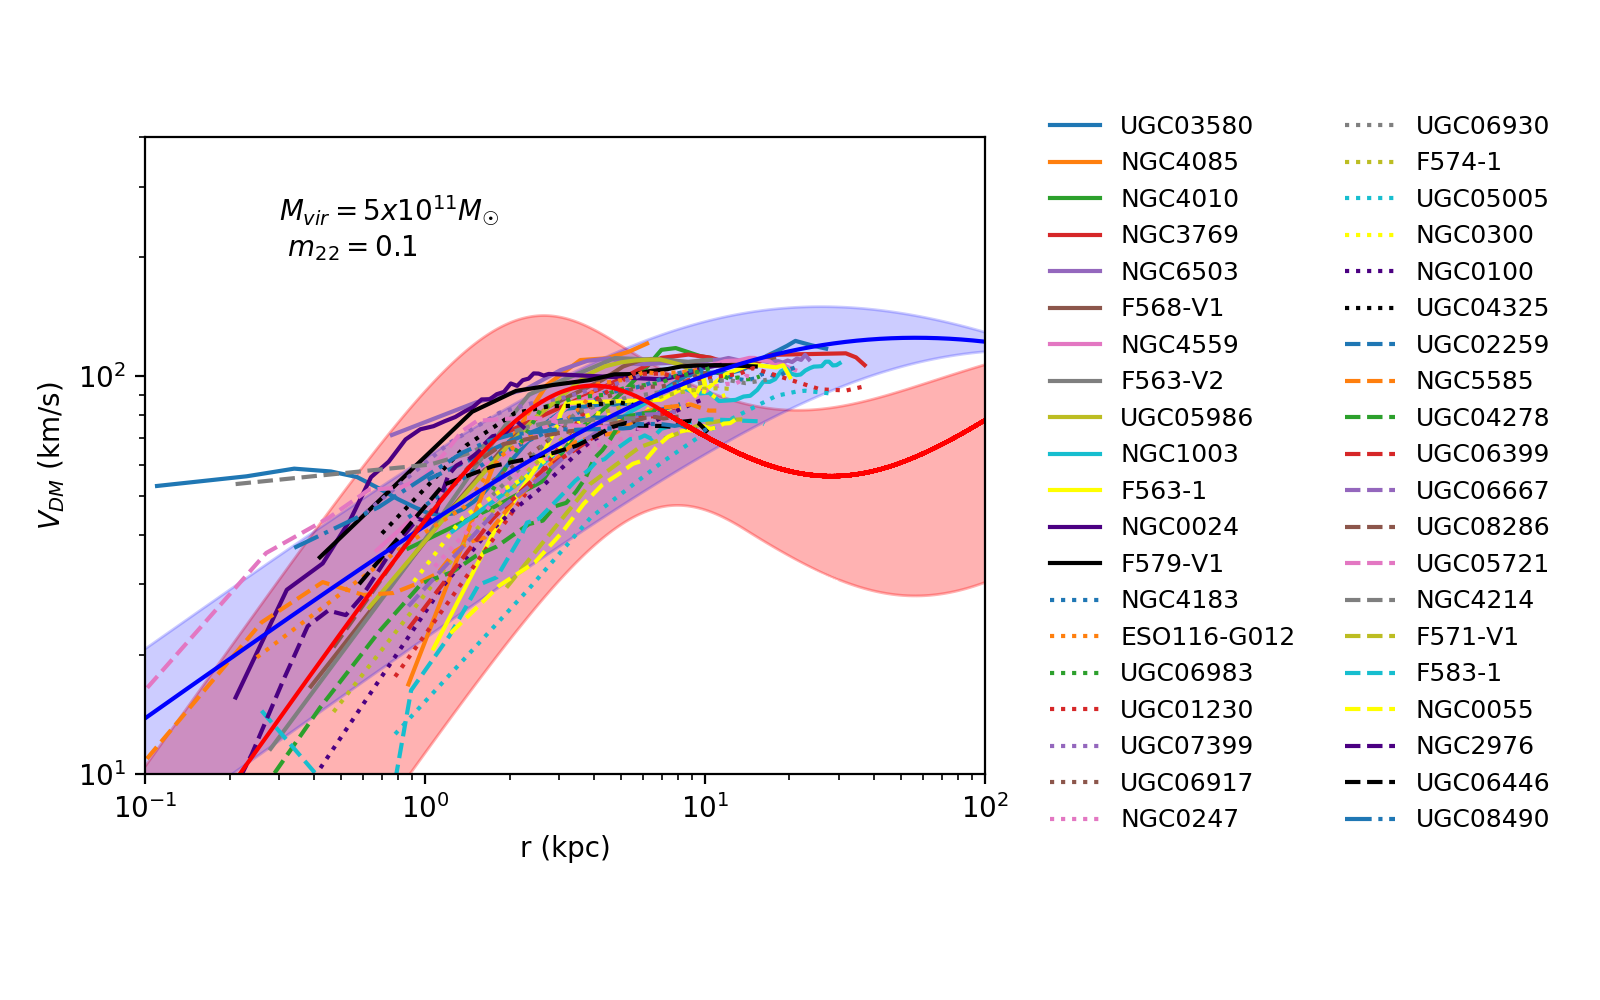
\includegraphics[scale=0.9, trim={0.5cm 1cm 0cm 1cm}]{000_vs_SPARC_5_10_11.png}
\caption{Velocity distributions for galaxies with maximum velocities in the range $75 \leq v < 125\operatorname{kms}^{-1}$ in the SPARC database. Data at outer radii is limited for these galaxies, making it difficult to determine the overall characteristics of the profiles. The SPARC data is plotted along with theoretical NFW and ULDM profiles, assuming a virial mass of $5\times10^{11} \mathrm{M}_{\odot}$, $m_{22} = 0.1$, and $\pm 50 \%$ scatter in the ULDM core-halo mass relation and $\pm2\sigma$ scatter in NFW concentration. Galaxies in the legend are ordered from highest maximum velocity (top left) to lowest (bottom right).}\label{fig:low_v}
\end{figure*}



\section{Conclusions}\label{sec:conclusion}

While the ULDM model has gained attention in part because it is a candidate solution to  the CDM core-cusp problem, in some cases ULDM profiles can have higher densities than their NFW counterparts at observationally relevant radii in the interior of halos of $M \gtrsim 10^{12} \mathrm{M}_{\odot}$. However, given the apparent spread in the predicted ULDM core-halo mass relation \cite{Schive:2014hza}, there is a sizeable range of plausible central densities for a halo of any given mass and analyses of oscillations of the cores of ULDM halos on timescales much smaller than the relaxation time have also demonstrated significant fluctuations in central density \cite{Veltmaat:2018dfz}. These observations suggest that the theoretical core-halo mass relation of ULDM should not be interpreted too literally for any individual halo, but is best viewed as a statistical feature of halo formation. However, because of limited simulation data, the exact features of this statistical distribution remain poorly characterised at present. Nevertheless, it is clear that choosing a core mass at the lower end of the plausible range can mitigate the apparent worsening of the core-cusp discrepancy for ULDM halos.  

With the spread around the predicted core-halo relation in mind, comparison of theoretical ULDM and NFW profiles to photometric data from the SPARC database yields inconclusive results. While it is relatively easy to choose parameters to provide a superficial fit to certain subsets of data, these data often do not span suitably large radial ranges for a meaningful assessment of the relative success of the theoretical UDLM and NFW profiles. This is because the regions in which the theoretical profiles differ strongly are often the same regions for which little observational data exists. 

We suggest, therefore, that current theoretical models cannot be realistically said to be more strongly favoured or disfavoured by comparison with available data. Indeed, while one could perform a BIC analysis to distinguish between the two models, the lack of comprehensive data, and the high number of free parameters (the stellar mass to light ratio in the SPARC data/ the assumed virial mass of the galactic halos, the ULDM particle mass, the NFW concentration parameter, the UDLM soliton to NFW transition radius and the variation around the core-halo mass relation) would make such an analysis highly vulnerable to overfitting, and therefore not robust. Hence, we caution against premature assessments of the ability of either ULDM or CDM models to reproduce astrophysical data.

It is clear that more information, both from simulations and astrophysical observations, is required to fully explore the applicability of the ULDM model of dark matter. The parameter space used to describe ``typical'' ULDM halos appears to be larger than simple semi-analytical models would suggest, and must also ultimately include elements of baryonic feedback. Tightening the constraints on the plausible ULDM particle mass will also inform future investigations of this type \cite{Castellano:2019hdd, Lidz:2018fqo, Davoudiasl:2019nlo} Furthermore, a larger volume of photometric data with improved uncertainties covering a greater halo mass range and radius would be of tremendous benefit when testing dark matter scenarios, and can be expected from future surveys  \cite{Simon:2019kmm}. In addition, cosmological structure formation simulations for ULDM models continue to be an active area of research \cite{Lin:2018whl, Clough:2018exo, Mocz:2015sda}, which will improve the clarity of predictions for these scenarios. This work, along with previous studies such as \cite{Bar2018acw}, which also tackled the core-halo mass relation and the fitting of semi-analytical profiles to galaxy data, emphasise the necessarily preliminary and tentative nature of all analyses of ULDM-derived rotation curves, and provides clear targets for future analyses. 



\begin{acknowledgements}
We acknowledge invaluable discussions with Jens Niemeyer, Shaun Hotchkiss, and Mateja Gosenca in completing this work. We also acknowledge support from the Marsden Fund of the Royal Society of New Zealand. This research was supported by use of the Nectar Research Cloud, a collaborative Australian research platform supported by the National Collaborative Research Infrastructure Strategy (NCRIS).

\end{acknowledgements}


\begin{appendix}

\begin{figure*}[t]
\centering
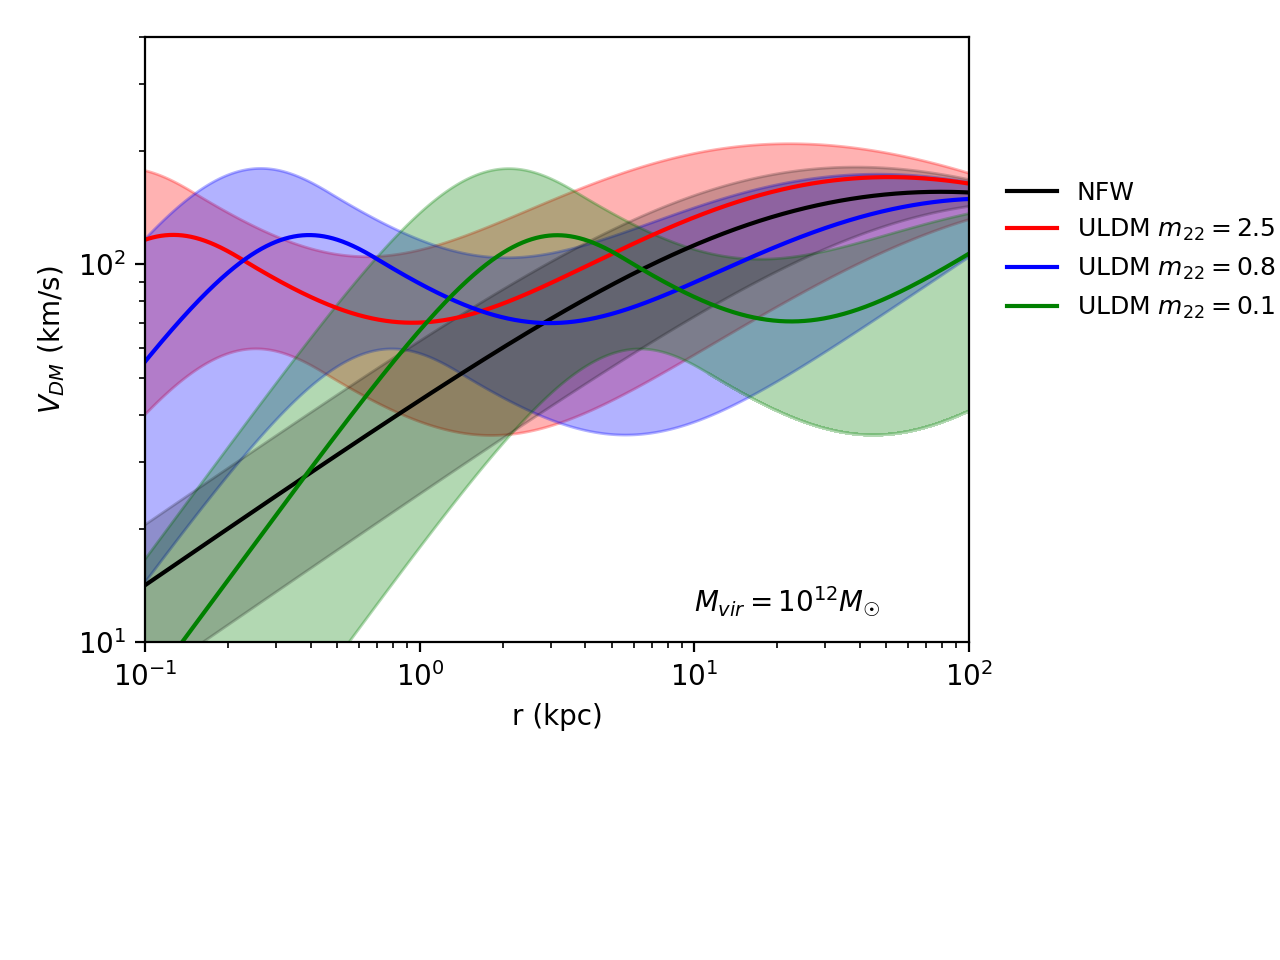
\includegraphics[scale = 0.8, trim={0cm 2.5cm 1cm 0cm}]{000_comp_10_12.png} 
\caption{Plot demonstrating the effect of changing the ULDM particle mass assumption on the velocity profiles for halos of mass $10^{12}\mathrm{M}_{\odot}$.}\label{fig:vel_5_10_11}
\end{figure*}

\section{ - Core-halo mass relation}\label{app:core-halo}

 The core-halo mass relation can be simply interpreted as the statement that the average internal velocity of a tracer mass in the core must be equal to the virial velocity of a tracer mass in the wider halo. If this were not the case, and instead the average velocity were higher within the core, these higher velocity particles would move outward, resulting in dynamical mass redistribution within the halo. During this process, the halo would not be in equilibrium and would thus not be virialised.

From the virial theorem we have that $E_K=-1/2 \ E_P$, where $E_K$ and $E_P$ represent kinetic and potential energies, respectively. Alternatively we can write:

\begin{equation}
    \frac{1}{2}M_{tot}v^2=\frac{1}{4}\frac{GM_{tot}^2}{R_{tot}},
\end{equation}
where $G$ is the gravitational constant, $M_{tot}$ and $R_{tot}$ are the total mass and radius, and $v^2$ is the mean of the squares of individual tracer velocities. Demanding that $v^2$ is the same for the core as for the total virialised halo allows us to then write
\begin{align}\label{eq:virial_cond}
    v^2&=\frac{GM_{\mathrm{vir}}}{2 R_{\mathrm{vir}}}=\frac{G M_{core}}{2 R_{core}}\nonumber\\
    &\rightarrow R_{core}=\frac{M_{core} R_{\mathrm{vir}}}{M_{\mathrm{vir}}}.
\end{align}
We know from the soliton scaling properties that $R_{core}\propto M_{core}^{-1}$, and since $M_{\mathrm{vir}}=4/3 \ \pi R_{\mathrm{vir}}^3 \Bar{\rho}$, we also have $R_{\mathrm{vir}} \propto M_{\mathrm{vir}}^{1/3}$. Hence, Equation \ref{eq:virial_cond} becomes
\begin{align}
    &R_{core}^2\propto \frac{R_{\mathrm{vir}}}{M_{\mathrm{vir}}}\nonumber\\
    &\rightarrow R_{core}^2\propto \frac{M_{\mathrm{vir}}^{1/3}}{M_{\mathrm{vir}}}\nonumber\\
    &\rightarrow R_{core}\propto\left(M_{\mathrm{vir}}^{-2/3}\right)^{1/2}\nonumber\\
    &\rightarrow R_{core}\propto M_{\mathrm{vir}}^{-1/3}.
\end{align}
With this scaling relation in mind, the constant of proportionality may be determined through analysis of simulated halos. 



\section{ - Impact of ULDM particle mass on halo velocity profiles}

Figure \ref{fig:vel_5_10_11} demonstrates the scale of the changes to the velocity profiles of theoretical ULDM halos under changes in the ULDM particle mass. Further work to constrain the plausible range of the particle mass will make comparisons of the ULDM and CDM models with astrophysical data more effective.

 
\end{appendix}

\bibliographystyle{pasa-mnras}
\bibliography{1r_lamboo_notes}

\end{document}
